\chapter{Results: Tropical Species Suitability Graphs} \label{AppendixI}

\begin{figure}[htb!]
\center
	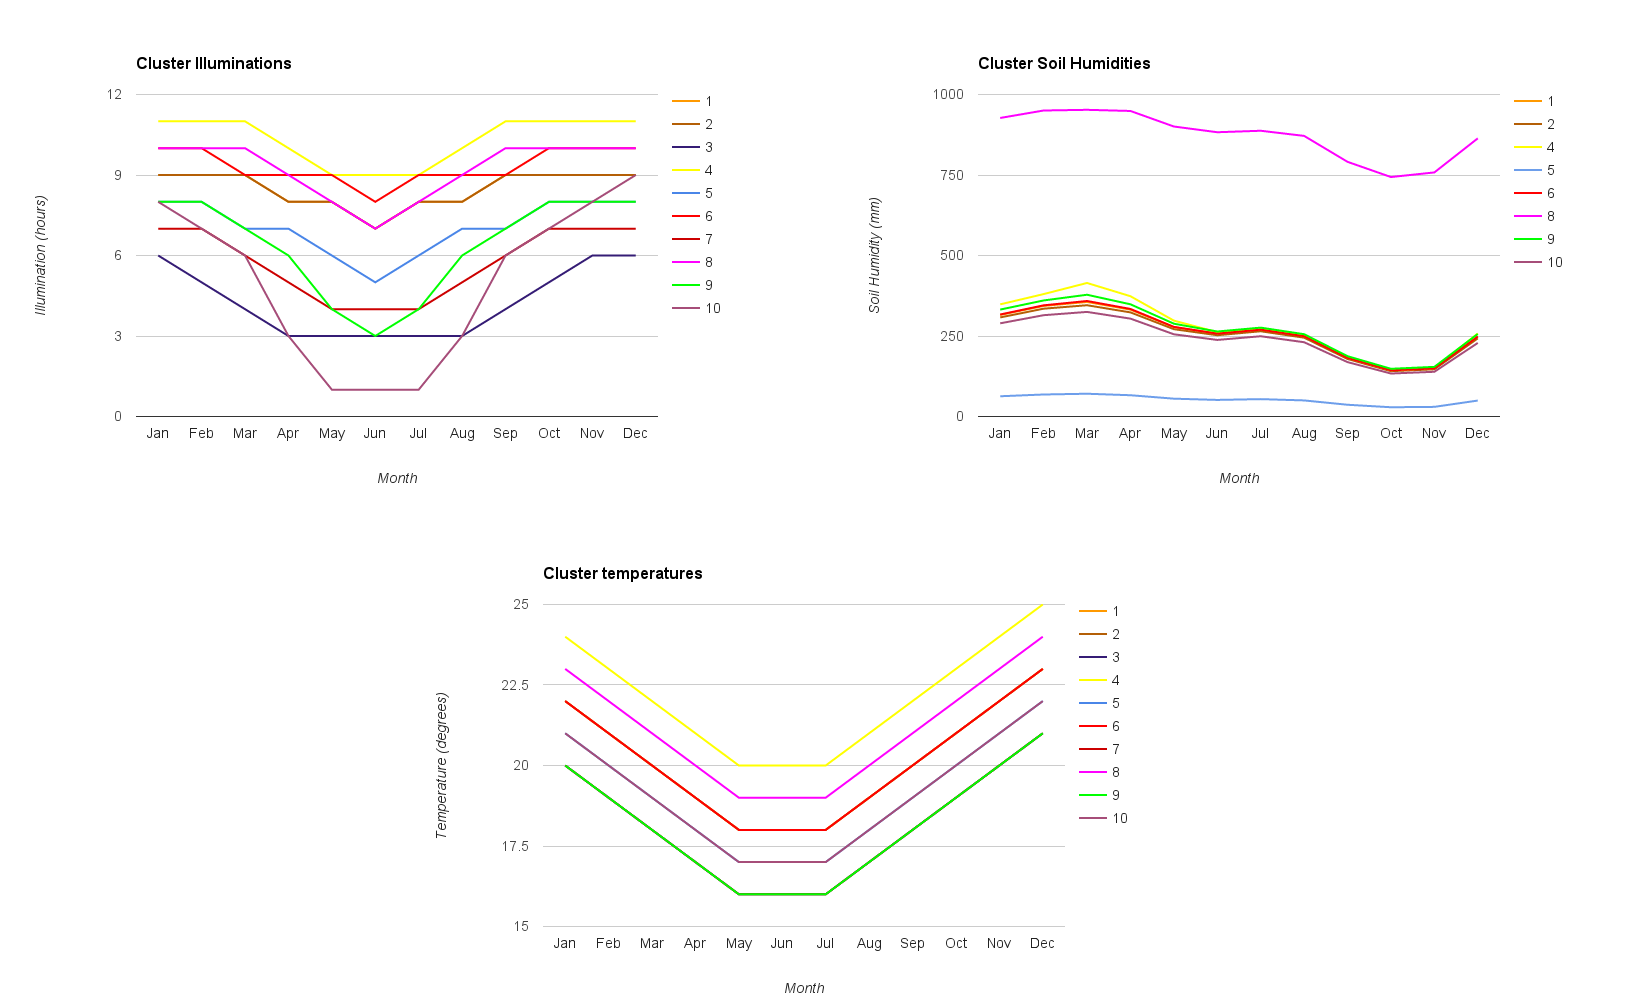
\includegraphics[height=\textheight-60pt,keepaspectratio]{results_tropical_clusters_hum_temp_illum.png}
	\caption{ \textit{Tropical rainforest: Monthly sun exposure (top), temperatures (middle) and soil moistures (bottom) for each terrain cluster. Note that soil humidity data is removed for clusters (3 and 7) as the corresponding values are too small.}}
	\label{fig:results_tropical_cluster_hum_temp_illum}
\end{figure}

\begin{figure}[htb!]
\center
	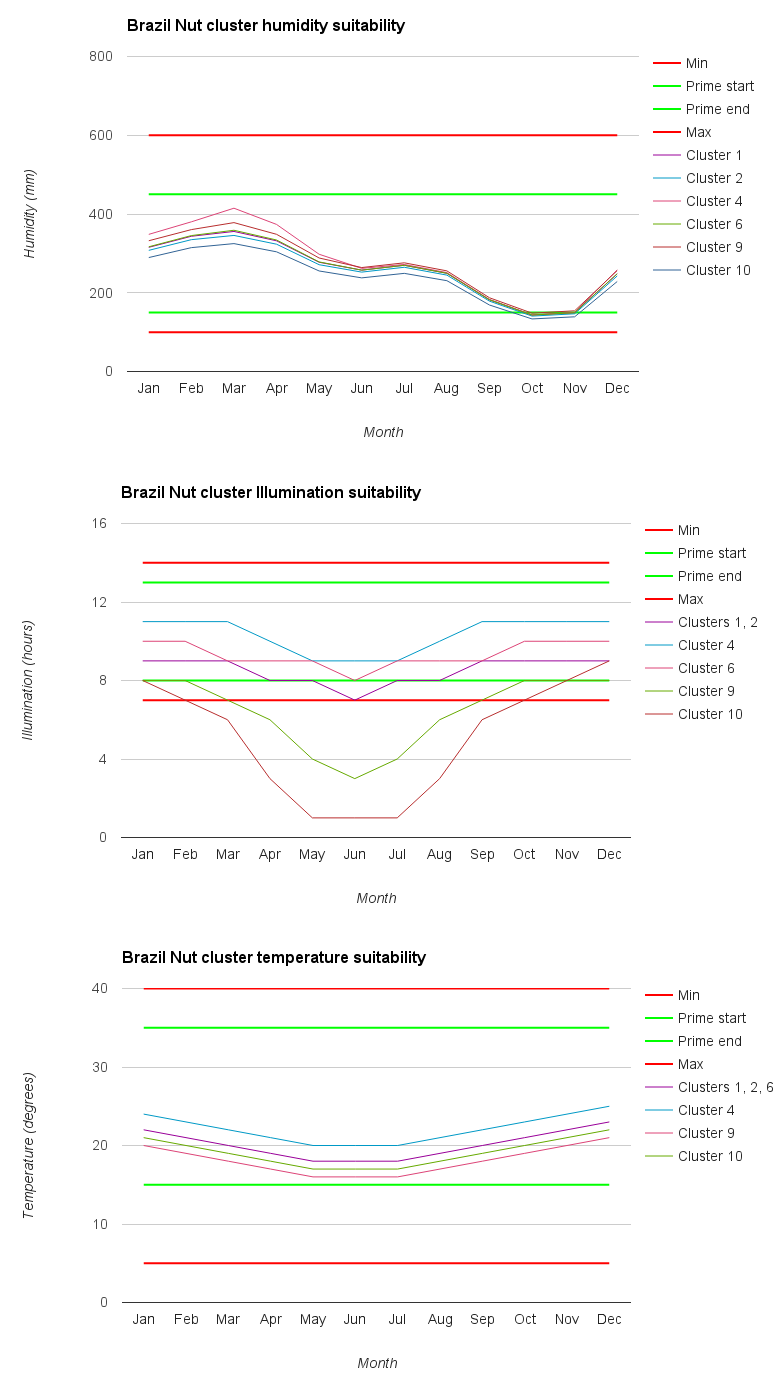
\includegraphics[height=\textheight-100pt,keepaspectratio]{brazil_nut_suitability.png}
	\caption{ \textit{Tropical rainforest: Brazil nut suitability to clusters 1, 2, 4, 6, 9 and 10 in terms of soil moisture (top), illumination (middle) and temperature. The thick green lines and red lines delimit the species prime range and absolute limits, respectively.} }
	\label{fig:results_tropical_brazil_nut_suitability}
\end{figure}

\begin{figure}[htb!]
\center
	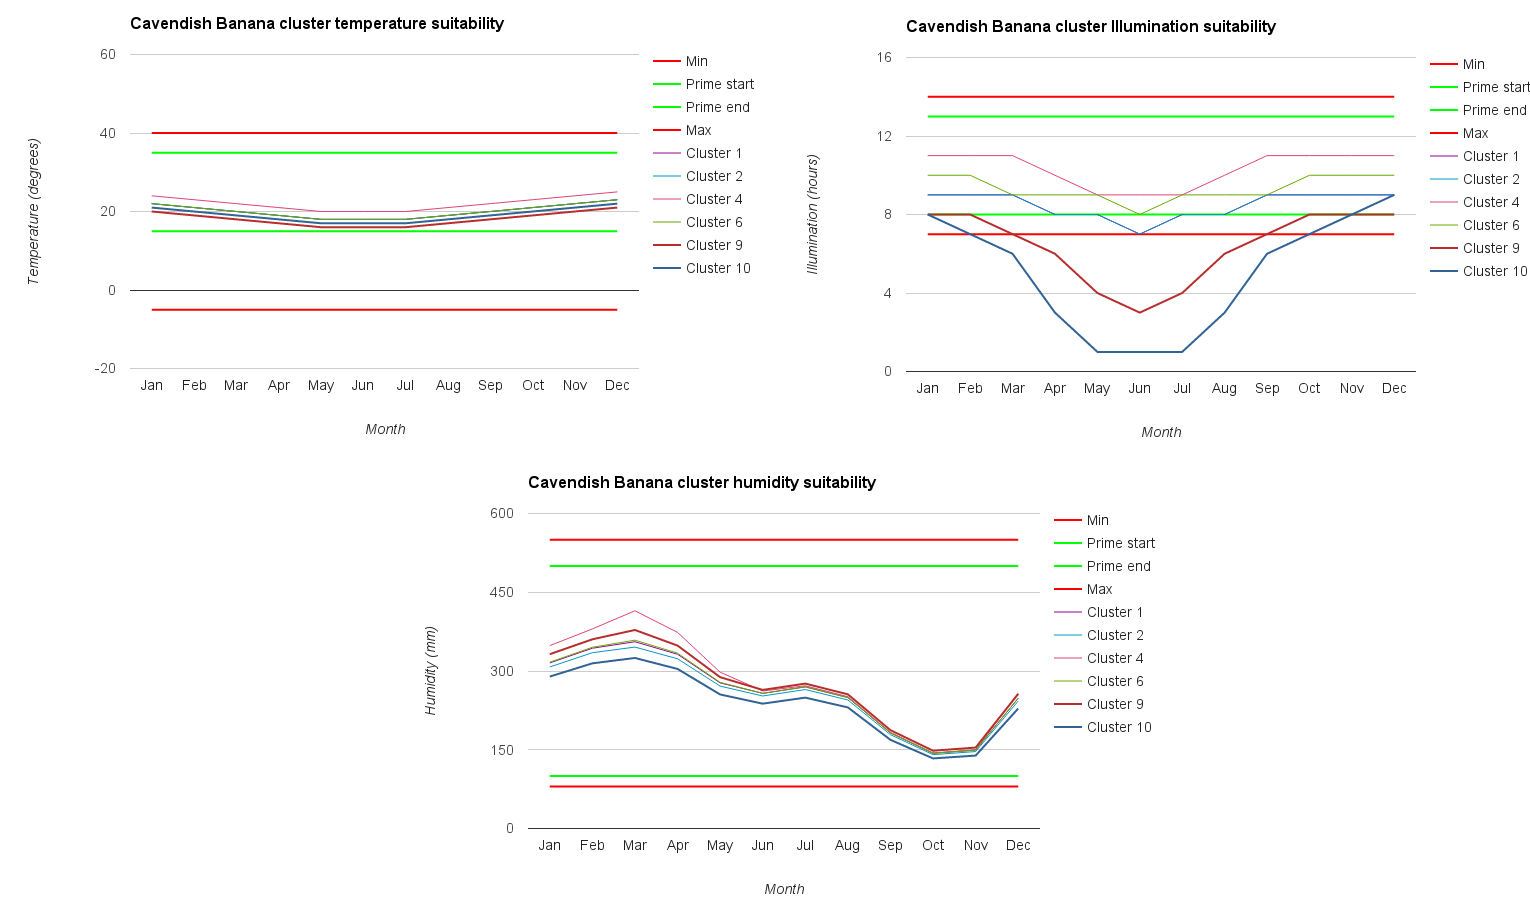
\includegraphics[height=\textheight-100pt,keepaspectratio]{cavendish_banana_suitability.png}
	\caption{ \textit{Tropical rainforest: Cavendish Banana suitability to clusters 1, 2, 4, 6, 9 and 10 in terms of soil moisture (top), illumination (middle) and temperature. The thick green lines and red lines delimit the species prime range and absolute limits, respectively.}}
	\label{fig:results_tropical_cavendish_banana_suitability}
\end{figure}

\begin{figure}[htb!]
\center
	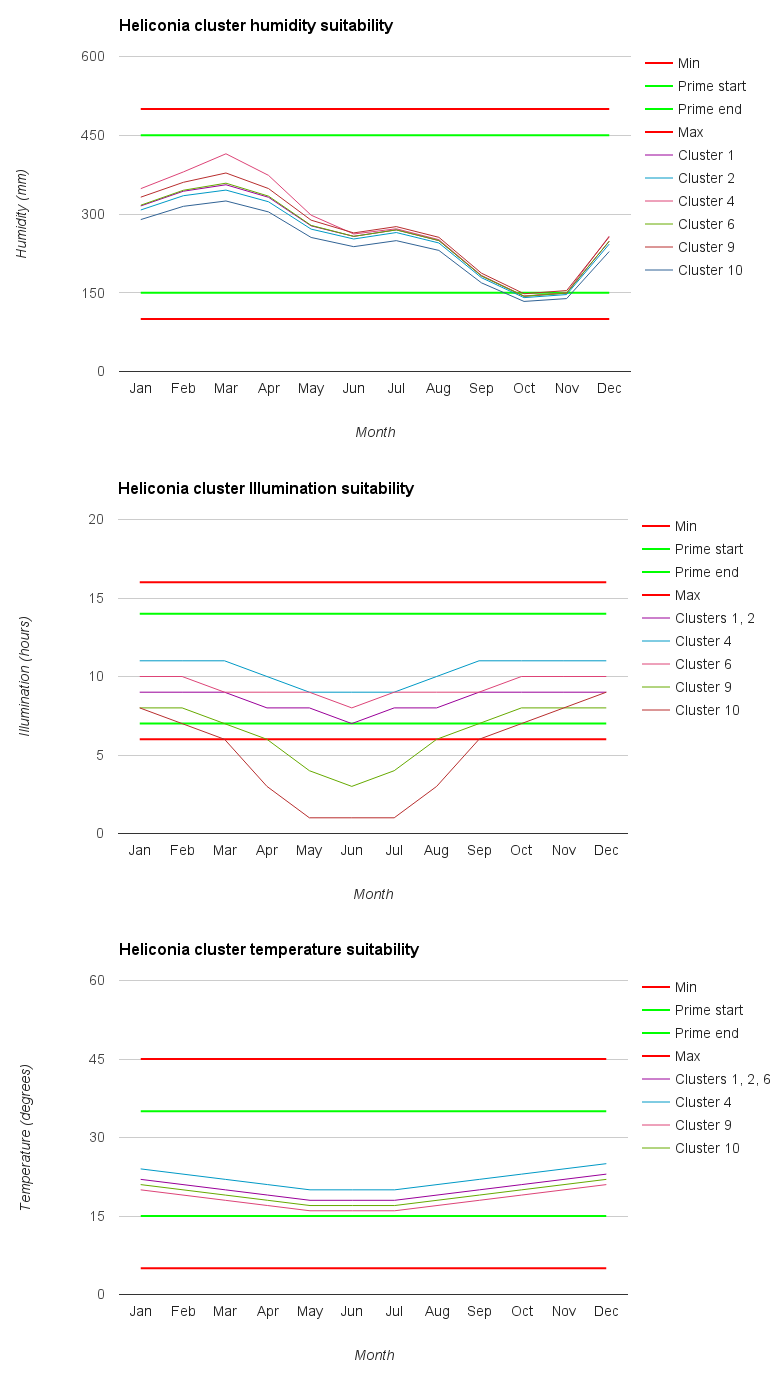
\includegraphics[height=\textheight-100pt,keepaspectratio]{heliconia_suitability.png}
	\caption{\textit{Tropical rainforest: Heliconia suitability to clusters 1, 2, 4, 6, 9 and 10 in terms of soil moisture (top), illumination (middle) and temperature. The thick green lines and red lines delimit the species prime range and absolute limits, respectively.}}
	\label{fig:results_tropical_heliconia_suitability}
\end{figure}

\begin{figure}[htb!]
\center
	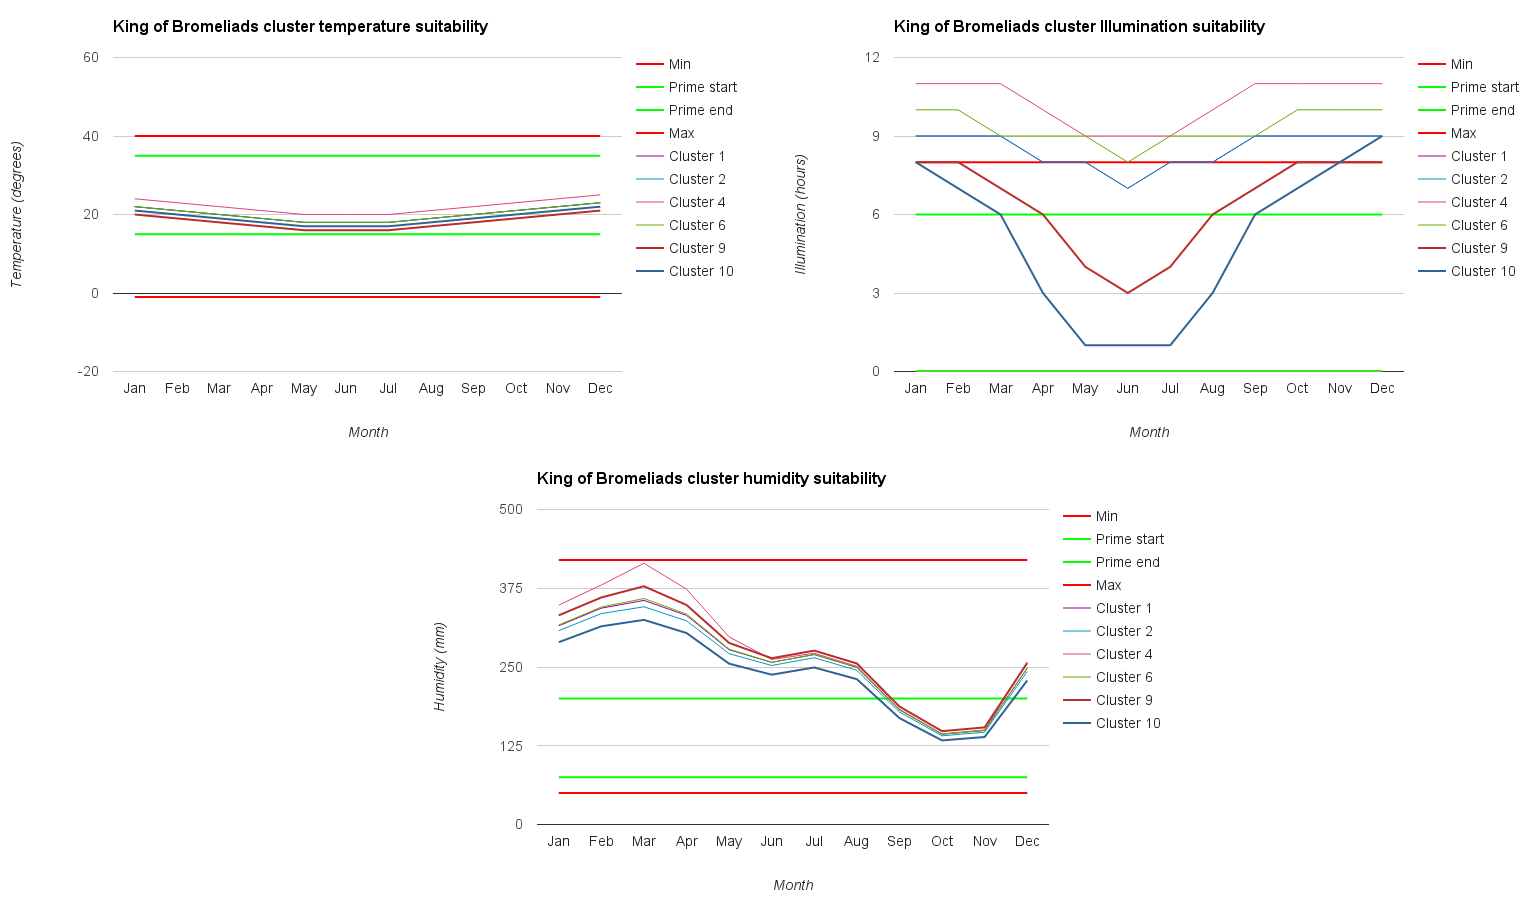
\includegraphics[height=\textheight-100pt,keepaspectratio]{king_of_bromeliads_suitability.png}
	\caption{ \textit{Tropical rainforest: King of Bromeliads suitability to clusters 1, 2, 4, 6, 9 and 10 iin terms of soil moisture (top), illumination (middle) and temperature. The thick green lines and red lines delimit the species prime range and absolute limits, respectively. Note that because the king of bromeliads is a shade-loving species, the minimum illumination line is not present as it is overlapped by the start of prime range line.}}
	\label{fig:results_tropical_king_of_bromeliads_suitability}
\end{figure}

\begin{figure}[htb!]
\center
	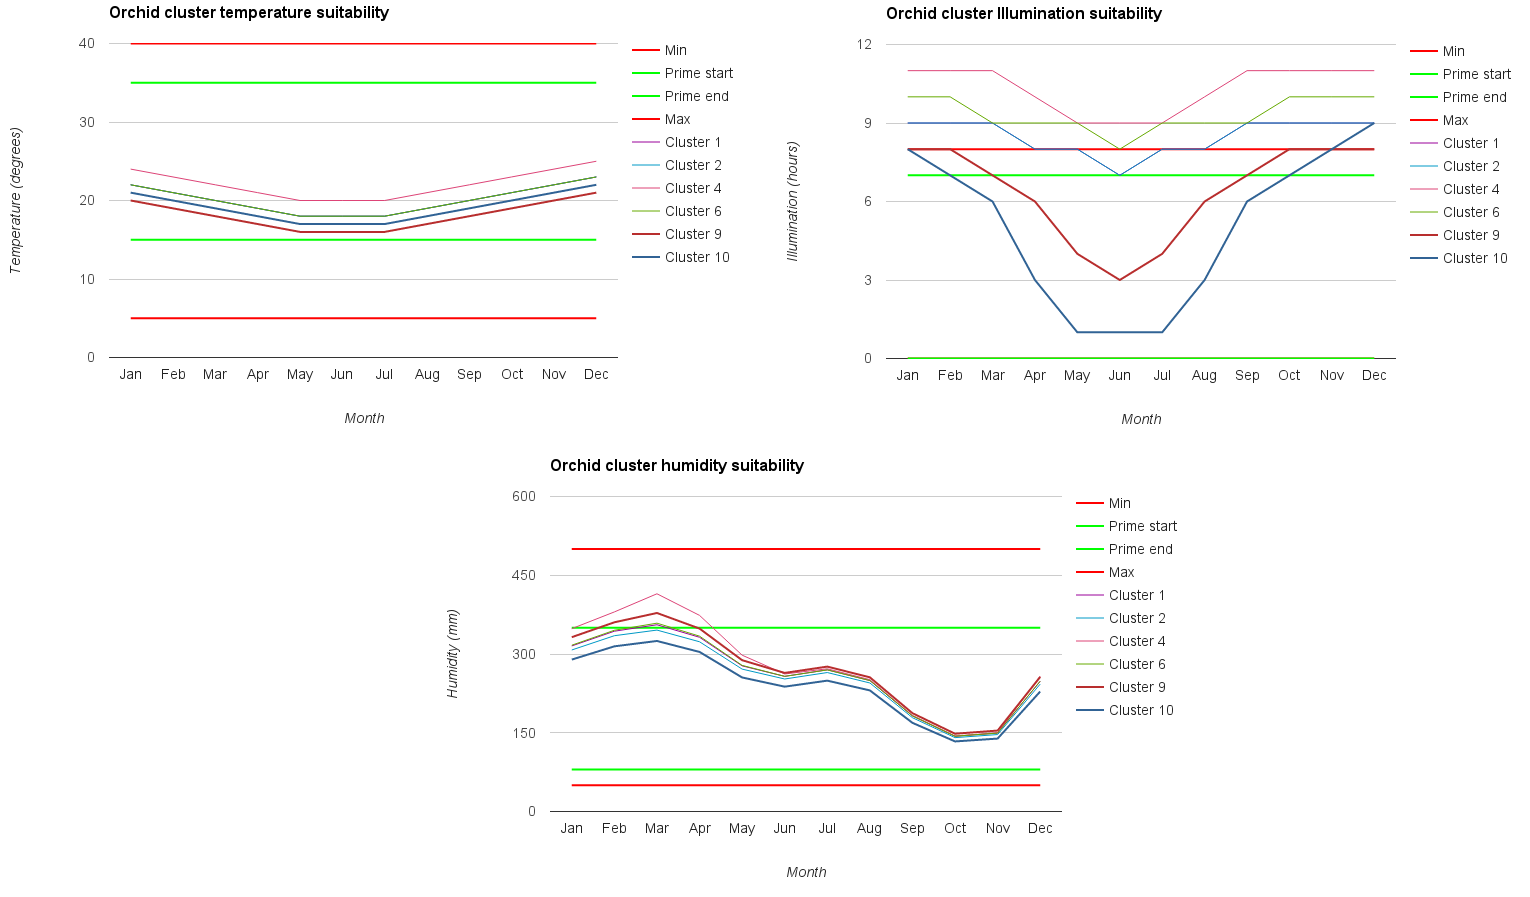
\includegraphics[height=\textheight-100pt,keepaspectratio]{orchid_suitability.png}
	\caption{ \textit{Tropical rainforest: Orchid suitability to clusters 1, 2, 4, 6, 9 and 10 in terms of soil moisture (top), illumination (middle) and temperature. The thick green lines and red lines delimit the species prime range and absolute limits, respectively. Note that because the king of bromeliads is a shade-loving specie, the minimum illumination line is not present as it is overlapped by the start of prime range line.}}
	\label{fig:results_tropical_orchid_suitability}
\end{figure}